\documentclass[brazil,ruledheader]{abntifes}
%\documentclass[brazil,twoside,ruledheader]{abntifes}
\usepackage[T1]{fontenc} 
%\usepackage[latin1]{inputenc}
\usepackage[utf8]{inputenc}
\usepackage[brazil]{babel}
\usepackage[]{algorithm2e}
\usepackage{pslatex}
\usepackage{url}
\usepackage{fancyhdr}
\usepackage{graphicx}
\usepackage{amsmath, amsthm, amssymb}
\usepackage{exercise}
\usepackage{makeidx}
\usepackage{setspace}
\usepackage{multicol}    
\usepackage{upquote}
\usepackage{graphicx}
\usepackage{float}
\usepackage{epigraph}

\usepackage{listings}

\lstset{numbers=left, stepnumber=5, firstnumber=1, numberstyle=\tiny, extendedchars=true, breaklines=true, frame=tb, basicstyle=\footnotesize, stringstyle=\ttfamily, showstringspaces=false }

%\makenomenclature

% Para listar programas em C# 
\lstdefinelanguage{cs}
  {morekeywords={abstract,event,new,struct,as,explicit,null,switch
		base,extern,object,this,bool,false,operator,throw,
		break,finally,out,true,byte,fixed,override,try,
		case,float,params,typeof,catch,for,private,uint,
		char,foreach,protected,ulong,checked,goto,public,unchecked,
		class,if,readonly,unsafe,const,implicit,ref,ushort,
		continue,in,return,using,decimal,int,sbyte,virtual,
		default,interface,sealed,volatile,delegate,internal,short,void,
		do,is,sizeof,while,double,lock,stackalloc,
		else,long,static,enum,namespace,string, },
	  sensitive=false,
	  morecomment=[l]{//},
	  morecomment=[s]{/*}{*/},
	  morestring=[b]",
}

\newcommand{\AUTOR}{João Pedro Souza Homem}
\newcommand{\SEGUNDOAUTOR}{}
\newcommand{\ORIENTADOR}{Marlan Kulberg}
\newcommand{\COORIENTADOR}{}
\newcommand{\TITULO}{Aplicação tempo-real com NodeJS - Chat por localização geográfica}
\newcommand{\CURSO}{Tecnólogo em Tecnologia da Informação e da Comunicação}
\newcommand{\GRAU}{Tecnólogo em Tecnologia da Informação e da Comunicação}
% \newcommand{\GRAU}{Tecnólogo em Análise e Desenvolvimento de Sistemas}
\newcommand{\INSTITUICAO}{Faculdade de Educação Tecnológica do Estado do Rio de Janeiro Faeterj/Petrópolis}
\newcommand{\ANO}{Dezembro, 2016}
\newcommand{\DATA}{12 de 12 de 2016}
\newcommand{\LOCAL}{Petrópolis - RJ}
\newcommand{\epigrafe}{\vspace{1cm}{\raggedright\par\sffamily\slshape\par}}
\begin{document}

\autor{\AUTOR}
\titulo{\TITULO}
\orientador{\ORIENTADOR}
\coorientador{\COORIENTADOR}

\comentario{Trabalho de Conclusão de Curso apresentado à Coordenadoria do Curso de \CURSO\
	    da \INSTITUICAO , como requisito parcial para obtenção do título de \GRAU .}

\instituicao{\INSTITUICAO}
\curso{\CURSO}
\governo{Governo do Estado do Rio de Janeiro}
\secretaria{Secretaria de Estado de Ciência e Tecnologia}
\fundacao{Fundação de Apoio à Escola Técnica}
\cpti{Centro de Educação Profissional em Tecnologia da Informação}
\local{\LOCAL}
\data{\ANO}

\capa

\folhaderosto

% Ficha Catalográfica
%\begin{figure}
%\includegraphics[width=11cm]{FichaCatalografica.pdf}
%\end{figure}

% Folha de Aprovação
\newpage
\vfill 
\null
\begin{center}
{\Huge {\bfseries\itshape Folha de Aprovação}}\\[3cm]
\begin{espacoduplo}
Trabalho de Conclusão de Curso sob o título \textit{``\TITULO''},
defendida por \AUTOR\ e aprovada em \DATA, em \LOCAL, pela banca examinadora constituída pelos
professores: \setlength{\ABNTsignthickness}{0.4pt}
\end{espacoduplo}
\setlength{\ABNTsignthickness}{0.4pt}

% ou inserir a página assinada e escaneada aqui
%\begin{figure}
%\includegraphics[]{Fo	lhaAprovacao.pdf}
%\end{figure}


\assinatura{Prof. \ORIENTADOR\\ Orientador} 
\assinatura{Prof. Banca Interna \\ \INSTITUICAO} 
\assinatura{Prof. Banca Interna \\ \INSTITUICAO} 
%\assinatura{Prof. Banca Externa \\ Instituto do membro externo}

\end{center}


% Folha do Termo de Compromisso
\newpage

\vfill 
\null
\begin{center}
{\Huge {\bfseries\itshape Declaração de Autor}}\\[3cm]
\begin{espacoduplo}
Declaro, para fins de pesquisa acadêmica, didática e tecnico-científica, que o presente Trabalho de Conclusão
de Curso pode ser parcial ou totalmente utilizado desde que se faça referência à fonte e aos autores.
\end{espacoduplo}
\setlength{\ABNTsignthickness}{0.4pt}
\assinatura{\AUTOR}
Petrópolis, em \DATA
\end{center}

\chapter*{Agradecimentos}
Agradeço a todos que de forma direta ou indireta contribuíram para a elaboração deste trabalho através do investimento em minha capacitação, compartilhamento de conhecimento, disponibilização de ferramentas e componentes para desenvolvimento de \textit{softwares}, entre outros não menos importantes.

Dentre todos os relacionados a este agradecimento, gostaria especialmente de agradecer a toda comunidade \textit{open-source}, da qual pude usufruir de diversos recursos que viabilizaram a implementação da aplicação abordada neste documento. A iniciativa \textit{open-source} abre muitos caminhos para a inovação e inclusão na área de desenvolvimento de \textit{softwares} e deve ser incentivada e reconhecida, atribuindo-se os devidos méritos a cada um que adere a iniciativa em seus projetos.
\vfill 
\null

\begin{center}
{\Huge {\bfseries\itshape Epígrafe}}\\[3cm]
\vspace{15cm}
\end{center}

\begin{espacoduplo}
\end{espacoduplo}

% Epigrafe
\epigraph{"Faça-se simples com ideias muito complicadas"}{(JoPaseho)}

% Resumo
\begin{resumo}
Texto


\end{resumo}

% Abstract
\begin{abstract}
Resumo em inglês ... "Não é obrigadorio"
\end{abstract}
\listoffigures

\listoftables

%Lista de abreviaturas
\newpage

\vfill 
\null
\begin{center}
	{\Huge {\bfseries\itshape Lista de Abreviaturas}}\\[3cm]
\end{center}

\begin{espacoduplo}
	\begin{description}
		\item[PUB/SUB] Publish/Subscription
		\item[SQL] Structured Query Language
		\item[NoSQL] Not Only Structured Query Language
	\end{description}
\end{espacoduplo}

\tableofcontents{}

% Capítulo
\chapter{Introdução}
Os avanços da tecnologia em conjunto com a internet têm ditado aos seus usuários novas formas de consumo de dados e informações. Além disto, um assunto tem ganhado cada vez mais destaque no provimento de dados na rede: a periodicidade. A inclusão dos meios tecnológicos no cotidiano das pessoas e o grande aumento do volume de dados gerados têm desenvolvido uma nova tendência de informações instantâneas, o que nos leva a elaborar meios para atender a esta nova demanda.

Alguns questionamentos aos modelos atuais de consumo de dados,  apesar de bem sucedidos em diversas áreas, surgem como uma necessidade ainda maior pelo consumo de informações. O \textit{e-mail}, tradicional meio de comunicação entre pessoas, oferecendo uma boa razão de confiabilidade e formalidade, já é questionado por \textit{startups} \cite{startup-email-innovation1} \cite{startup-email-innovation2} que acreditam no futuro da \textit{web} em tempo real.

% Seção
\section{Motivação} 
As aplicações de tempo real estão surgindo como requisitos de muitos dos novos sistemas em desenvolvimento, e buscam atender consumidores que já possuem em seus negócios a necessidade da informação imediata. Neste trabalho será desenvolvido uma aplicação que explora de forma bem específica essa necessidade da troca de informações entre usuário e aplicação em tempo real.

A aplicação desenvolvida será um \textit{web chat} de comunicação por texto baseado em localização geográfica. As duas principais características do projeto, comunicação por texto e localização geográfica, trazem para si aspectos modernos, que exigem a utilização de ferramentas e técnicas atuais de desenvolvimento para a \textit{web}. Deve-se levar em consideração diversos conceitos, como compatibilidade, escalabilidade, infraestrutura de sistemas, entre outros. Tudo isto serve como motivação para atualização e aprendizado de diversos tópicos relacionados ao desenvolvimento de \textit{softwares}.   

% Seção
\section{Objetivos}
A finalidade do projeto será demonstrar como pode ser feita a transferência de dados em tempo real entre servidores e clientes. Para isto, será feita a implementação de uma aplicação que irá realizar a comunicação por texto entre usuários, que serão localizados para comunicação através de localização geográfica em um mapa terrestre real.

O produto mínimo viável da aplicação será elaborado para um ambiente de testes local, não oferecendo um fluxo completo de funcionamento dos servidores em ambiente de produção, nem do fluxo de utilização de um usuário comum em sua interface. Abordaremos apenas alguns conceitos sobre escalabilidade e infraestrutura da aplicação em ambiente de produção, assim como apenas algumas funcionalidades necessárias para interação na interface gráfica.

Será explicado com mais clareza os problemas que acercam este projeto no tópico "Problematização", abordando especificamente quais são os ideais de implementação de uma solução em tempo real que tem características semelhante a desenvolvida neste trabalho, levando em conta aspectos como produto e serviço, já que ideologicamente um software é feito para realizar uma ou mais funções para um ou mais usuários, mas como citado, o foco é demonstrar fundamentalmente o funcionamento deste tipo de aplicação, e não oferecer um produto ou serviço. A problematização irá se perfazer em torno do estudo de uma forma de se implementar uma solução de tempo real para a \textit{web} envolvendo duas funcionalidades de representatividade para a circunstância.

\chapter{Trabalhos Relacionados}
Com o objetivo de situar o presente trabalho em relação ao funcionamento da arquitetura e funcionalidades do sistema, analisamos alguns trabalhos que se assemelham em um ou mais aspectos da aplicação desenvolvida. Dentre estas, estão relacionadas propostas de implementação, que explicam o funcionamento da arquitetura de aplicações de tempo real, e também projetos que foram publicados como produto de mercado.

Será feita uma breve análise de cada uma das plataformas, sendo que algumas análises serão fundamentadas em sites que falam sobre o funcionamento destas, pois as mesmas não se encontram mais disponíveis para acesso. Contudo, são ferramentas que tentaram como produto final uma aplicação muito semelhante a desenvolvida como caso de estudo neste trabalho.

\section{Uber}
Iniciando a pesquisa sobre o desenvolvimento de uma aplicação de tempo real, foi buscada uma referência, que segundo estatísticas \cite{uber-statistics}, é considerada uma aplicação de grande escala. O Uber \cite{uber} é uma aplicação \textit{web} e \textit{mobile} que oferece serviços de transporte urbano privado através de pessoas que se disponibilizam a serem motoristas e estarem disponíveis na plataforma para alguma oferta de demanda.

Encontrou-se um site \cite{uber-how-scales} que fez-se de grande valia para o inicio da escolha das tecnologias que utilizamos para desenvolver a aplicação deste trabalho. A publicação fala sobre como era a arquitetura do sistema, para quais possibilidades ela foi pensada, e sobre a nova organização do sistema e quais tecnologias utilizam para suportar tamanha demanda \cite{uber-statistics}.

É notório ao longo do trabalho que a arquitetura aplicada para desenvolvimento da aplicação não se aproxima em muitos pontos da aplicada no Uber, mas após o estudo da publicação, fomos fomentados a pesquisar algumas das tecnologias utilizadas e como aplicá-las em nosso projeto. A principal influência retirada deste projeto foi a utilização do Redis como banco de dados em memória, e não diretamente uma influencia, mas uma consolidação de ideias, a utilização do NodeJS e um banco de dados NoSQL (Not Only Structured Query Language) \cite{nosql-advantages} para persistência dos dados.

As imagens \ref{fig:uber-main-interface} e \ref{fig:uber-payment-interface} mostram brevemente a interface do Uber. Na imagem \ref{fig:uber-main-interface} podemos observar a interface principal, e é possível notar a utilização do mapa, o qual nestes são contidos os carros próximos a uma localização, estes com suas posições geográficas atualizadas em tempo real devido ao fato de estarem se movimentando. Estas características representam bem algumas funcionalidades que serão implementadas na aplicação.

A imagem \ref{fig:uber-payment-interface} mostra a aplicação \textit{web} do Uber. Nesta é possível fazer o gerenciamento das contas de usuário em um formato mais cômodo e adequado para análise dos dados gerados através da utilização do aplicativo \textit{mobile}, como é mostrado na imagem \ref{fig:uber-payment-interface} um histórico detalhado de uma corrida, com trajetória realizada, horário, preços, entre outros.

\begin{figure}[H]
	\centering
	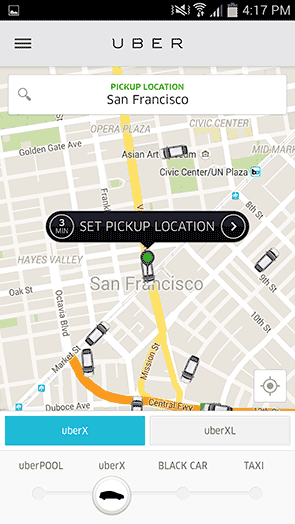
\includegraphics[scale=0.6]{imagens/uber.png}
	\caption{\small Interface principal do Uber Mobile.} Fonte: Referral SaaSquatch \cite{uber-imgs}
	\label{fig:uber-main-interface}
\end{figure}

\begin{figure}[H]
	\centering
	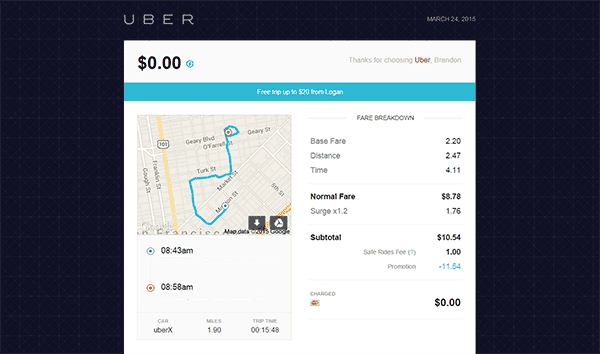
\includegraphics[scale=0.7]{imagens/uber2.png}
	\caption{\small Interface de pagamento do Uber Web.} Fonte: Referral SaaSquatch \cite{uber-imgs}
	\label{fig:uber-payment-interface}
\end{figure}

\section{Redis Publish-Subscribe (RedisMVA) }
Esta publicação \cite{redis-pubsub-redismva} faz parte de um projeto demonstrativo da utilização do padrão de comunicação pub/sub (Publish/Subscription), com um banco de dados NoSQL, chamado Redis. É abordada a implementação em NodeJS de um \textit{chat} de comunicação por texto, utilizando o padrão pub/sub para realizar a comunicação entre processos, onde os processos são as diversas instâncias que podem ser executadas de um mesmo servidor NodeJS distribuídos em diversos locais na internet.

O estudo desta publicação serviu como grande base de aprendizado para a elaboração da arquitetura do sistema que desenvolvemos, pois utilizava tecnologias atuais e que já tínhamos como plano para a implementação do nosso sistema, como citamos no caso do Uber. A utilização da linguagem de programação JavaScript, naturalmente traz um certo intimismo para quem já desenvolve para a \textit{web}, dado que ela pode ser considerada a linguagem da \textit{web} (\textit{client-side}), pois todos os maiores navegadores \textit{web} \cite{browsers-usage} utilizados no mundo interpretam a linguagem nativamente, sendo muito comum programadores voltados para a área já terem tido algum contato com a linguagem.

O autor da publicação disponibiliza todo o código fonte do projeto de demonstração com licença aberta, sendo assim, ele discorre sobre o tema de forma muito objetiva, apenas abordando em seu texto os pontos de interseção em que a implementação da comunicação pub/sub se insere. O texto oferece uma didática teórica de boa qualidade, demonstrando com diagramas e imagens da aplicação real, o funcionamento de cada passo do qual explica no documento.

A demonstração dos fluxos de dados que ocorrem no sistema ficam bem representadas com os diagramas, embora alguns destes fluxos não estejam implementados no sistema, como o balanceador de carga, visto que não era o foco de esclarecimento. É simples entender como a interface envia os dados para o servidor, que distribui os dados para os outros clientes conectados.

\section{Redis Pub-Sub (Rajaraodv)}
Esta publicação \cite{redis-pubsub-rajaraodv} fala sobre o mesmo assunto da citação anterior, que é a implementação de um chat por texto utilizando NodeJS e banco de dados Redis, mas nesta publicação o autor é mais abrangente no quesito de infraestrutura e escalabilidade da aplicação, abordando todos os passos para uma implantação completa do sistema em um servidor.

O texto da publicação é muito explicativo, é possível até para os mais principiantes no assunto de aplicações de tempo real entenderem a implementação e a finalidade de cada passo relatado. O texto também conta com ilustrações dos fluxos de dados na aplicação e demonstrações do funcionamento da interface.

O que se pode extrair do conteúdo desta publicação além da anterior, é a implementação do balanceador de carga, em conjunto com o \textit{proxy} reverso Nginx (aplicação que controla como será feito o fluxo de dados de fora para dentro da rede de servidores), o conceito de \textit{sticky sessions} (técnica que grava nas requisições de um cliente informações sobre servidor de origem da sessão) para traçar requisições a um mesmo servidor, e a integração do sistema em um servidor na nuvem (conjunto de recursos computacionais na internet, dedicados a hospedar aplicações de diversos tipos). 

Após o estudo da publicação deste autor, utilizamos em nossa implementação a utilização do Nginx. Entendemos a ideia de centralizar a distribuição de conteúdo estático da aplicação, como a interface, e canalizar as conexões aos servidores através de um ponto em comum, facilitando assim o gerenciamento para futuras implementações de \textit{sticky sessions}, balanceamento de carga, reconexão em casos de \textit{scale-up} ou \textit{scale-out} dos servidores (aumento e diminuição do número de servidores), entre outros benefícios que este tipo de arquitetura pode prover para as aplicações modernas. Tudo isso aspira o rumo em que a tecnologia vem tomando com o crescimento exponencial de usuários, consumo de dados, globalização, entre outros, que contribuem para a necessidade de se construir sistemas que sejam distribuídos e escaláveis, alcançando altos desempenhos.

\section{FanMappr e RadiusIM}
O FanMappr \cite{fanmappr} e o RadiousIM \cite{radiusim} são aplicações baseadas em \textit{chat} por localização geográfica, mas que foram disponibilizadas como produto, com a proposta de criarem relações sociais através da busca de usuários por localização, ou seja, são redes sociais e tinham isso como proposta final. Após uma análise mais técnica nos dois últimos tópicos em relação ao desenvolvimento da aplicação, agora iremos analisar ferramentas que implementam como um produto, aplicações que tem funcionalidades semelhantes as do nosso projeto.

Encontramos o FanMappr e RadiusIM após algumas poucas pesquisas que buscavam especificamente produtos que tivessem funcionalidades muito próximas das que implementamos em nossa aplicação. O FanMappr é uma aplicação com interface e funcionalidades aparentemente modestas, navegando entre os poucos menus que possui, percebemos que as funcionalidades se restringem somente ao \textit{chat} por texto e a um mapa terrestre onde os usuários são localizados.

A imagem \ref{fig:fanmappr-principal} é uma captura de tela da aplicação \textit{web} do FanMappr. Nela é possível notar a simplicidade da aplicação, que não possui personalizações das ferramentas utilizadas, como o mapa, e não utiliza conceitos de responsividade, pois a captura de tela foi realizada em um monitor de 22 polegadas, e a interface da aplicação se manteve no mesmo formato utilizado para tela menores.

\begin{figure}[H]
	\centering
	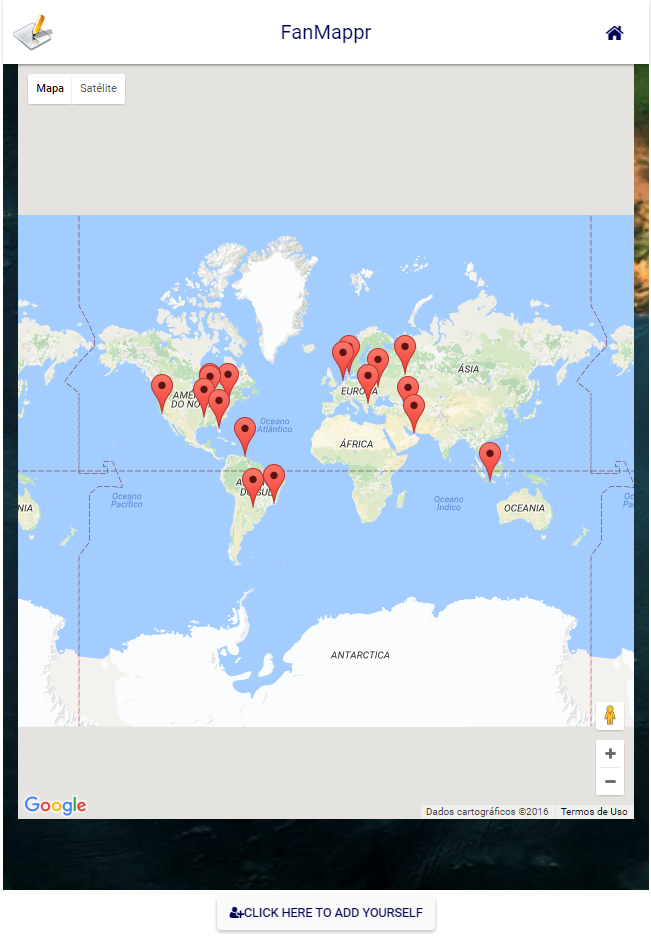
\includegraphics[scale=0.33]{imagens/fanmappr.png}
	\caption{\small Interface principal do FanMappr.} Fonte: Captura de tela
	\label{fig:fanmappr-principal}
\end{figure}

O RadiusIM não está mais disponível para acesso, mas encontramos um artigo \cite{radiusim} que possuía algumas imagens sobre a aplicação e uma breve explicação do seu funcionamento.

Foi possível notar que o RadiusIM também é muito semelhante com do FanMappr, apesar de parecer ter tido mais sucesso, nos anos 2000, presume-se que teve um investimento maior, pois possuía uma interface mais harmoniosa e funcionalidades que eram o de se esperar para sua época.

Podemos observar nas imagens \ref{fig:radiusim-principal} e \ref{fig:radiusim-chat} alguns detalhes de sua interface que demonstram um pouco da utilização do sistema. A imagem \ref{fig:radiusim-principal} \t mostra que de forma amigável ao usuário, a interface fornece os dados de sua localização, marcação no mapa, e uma série de pessoas nas proximidades e suas respectivas imagens de perfil. Na imagem \ref{fig:radiusim-chat} podemos ver a janela de chat 

\begin{figure}[H]
	\centering
	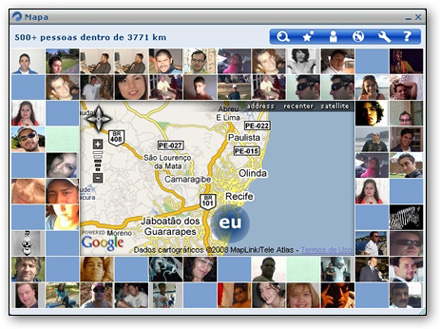
\includegraphics[scale=0.9]{imagens/radiusim.jpg}
	\caption{\small Interface principal do RadiusIM.} Fonte: wwwhats new \cite{radiusim}
	\label{fig:radiusim-principal}
\end{figure}

\begin{figure}[H]
	\centering
	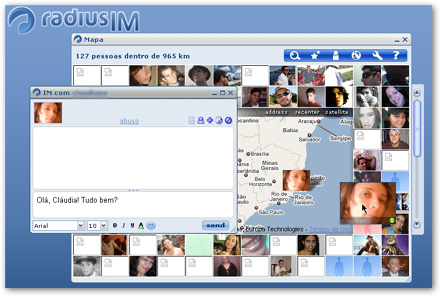
\includegraphics[scale=0.9]{imagens/radiusim2.jpg}
	\caption{\small Janela de \textit{chat} do RadiusIM.} Fonte: wwwhats new \cite{radiusim}
	\label{fig:radiusim-chat}
\end{figure}

É interessante perceber que estas aplicações não tiveram grande sucesso colocando como produto final uma ferramenta de comunicação com funcionalidades semelhantes a que iremos implementar, o que nos leva a interpretar que a \textit{web} em tempo real não é uma inovação a qualquer custo. É importante considerar que as melhorias que se pode ter com informações em tempo real devem ser mensuradas, e ela é apenas mais uma opção que está ganhando mais importância com as demandas que estão surgindo.

\section{Snapchat, Happn, Tinder e afins}
Neste tópico iremos fazer uma análise, mais filosófica do que técnica, sobre a utilização de aplicações de tempo real na vida dos usuários, pois achamos interessante fundamentar onde estão se rompendo os limites para a necessidade de aplicações deste tipo, e gostaríamos de ressaltar que Snapchat \cite{snapchat}, Happn \cite{happn} e Tinder \cite{tinder} foram escolhas que achamos que representam um grupo de aplicações com características próximas, mas que para muitas outras aplicações existentes, caberiam-se a mesma análise.

A seguir foi feita a síntese de uma citação \cite{notnotcitricsquid} que nos traz algumas importantes informações sobre a opinião de um usuário comum:

\begin{quote}
	\small "Há uma diferença fundamental entre chat baseado em localização e aplicativos de chat, como o Snapchat. O Snapchat mudou como as pessoas se comunicam, não mudou como elas encontram as pessoas para se comunicar.
	
	A localização em si não define quem somos ou o que gostamos, as pessoas buscam se comunicar com pessoas que possuam outros tipos de afinidades, e estas é que devem ser exploradas para se criar um aplicativo que seja interessante." 
	
	(Síntese de "Do location based chat apps start trending again?" \cite{notnotcitricsquid}, NOTNOTCITRICSQUID, 2012)
\end{quote}

A resposta a pergunta do tópico expressa uma opinião que condiz com alguns pontos que pudemos notar ao longo do conteúdo apresentado até aqui, que se relacionam com como as aplicações tem obtido sucesso na inserção da experiência de tempo real na vida dos usuários mais comuns, e aplicações como o FanMappr e o RadiusIM não alcançaram o mesmo resultado. Snapchat, Happn e Tinder são aplicações que utilizam localização geográfica em muitas de suas funcionalidades, mas trabalham a experiência do usuário com este tipo de funcionalidade de uma forma que preserva conceitos como os abordados na citação anterior, e este é um ponto que acreditamos ser o diferencial para a aceitação das ferramentas deste tipo, pelo fato de não infringir algumas barreiras que existem na interação humana com o mundo virtual.


%===================================================================================
%\backmatter
%===================================================================================

%\bibliography{monografia}{}
%\bibliographystyle{abnt-alf}

% OUTRA FORMA DE CRIAR A BIBLIOGRAFIA:
\begin{thebibliography}{9}

%
%	Capitulo 1 - Introdução
%
\bibitem{startup-email-innovation1}Liveclicker Delivers Dynamic Messaging Capability with RealTime Email Solution. Disponível em: \url{http://www.destinationcrm.com/Articles/CRM-News/CRM-Featured-News/Liveclicker-Delivers-Dynamic-Messaging-Capability-with-RealTime-Email-Solution-97439.aspx}.
Acesso em: 19 Out. 2016.

\bibitem{startup-email-innovation2}Liveclicker RealTime Email Solution. Disponível em: \url{http://www.realtime.email/}.
Acesso em: 19 Out. 2016.

\bibitem{uber-statistics}50 Amazing Uber Statistics (October 2016). Disponível em: \url{http://expandedramblings.com/index.php/uber-statistics/}.
Acesso em: 20 Out. 2016.

\bibitem{uber}Uber. Disponível em: \url{https://www.uber.com/}.
Acesso em: 20 Out. 2016.

\bibitem{uber-how-scales}How Uber Scales Their Real-Time Market Platform. Disponível em: \url{http://highscalability.com/blog/2015/9/14/how-uber-scales-their-real-time-market-platform.html}.
Acesso em: 20 Out. 2016.

\bibitem{redis-pubsub-redismva}Redis Publish-Subscribe (RedisMVA). Disponível em: \url{https://github.com/sayar/RedisMVA/blob/master/module6_redis_pubsub/README.md#redis-publish-subscribe}.
Acesso em: 20 Out. 2016.

\bibitem{browsers-usage}Web browsers usage table. Disponível em: \url{http://caniuse.com/usage-table}.
Acesso em: 20 Out. 2016.

\bibitem{redis-pubsub-rajaraodv}Redis Pub/Sub (Rajaraodv). Disponível em: \url{https://github.com/rajaraodv/redispubsub}.
Acesso em: 20 Out. 2016.

\bibitem{fanmappr}FanMappr. Disponível em: \url{http://h.fanapp.mobi/modules/fanmappr/fanmappr.php?fid=1056666}.
Acesso em: 20 Out. 2016.

\bibitem{radiusim}RadiusIM – Social Messenger Com Busca Por Geotagging. Disponível em: \url{http://br.wwwhatsnew.com/2008/09/radiusim-%E2%80%93-social-messenger-por-com-busca-por-geotagging/}.
Acesso em: 20 Out. 2016.
	
\bibitem{notnotcitricsquid}NOTNOTCITRICSQUID. Do location based chat apps start trending again?. Disponível em: \url{https://www.reddit.com/r/startups/comments/1tkc3f/do_location_based_chat_apps_start_trending_again/}.
Acesso em: 21 Out. 2016.

\bibitem{snapchat}Snapchat. Disponível em: \url{https://www.snapchat.com/}.
Acesso em: 21 Out. 2016.

\bibitem{tinder}Tinder. Disponível em: \url{https://www.gotinder.com/}.
Acesso em: 21 Out. 2016.

\bibitem{happn}Happn. Disponível em: \url{https://www.happn.com/}.
Acesso em: 21 Out. 2016.

\end{thebibliography}


\anexo
\end{document}